\documentclass{report}
\usepackage[utf8]{inputenc}
\usepackage[romanian]{babel}
\usepackage{float}
\usepackage{graphics}
\usepackage{graphicx}
\title{Vedere artificial\u a pentru Vehicule \\ Documenta\c tie \\ Quizzy [ZipGrade-like app]}
\author{Botescu Mihai: \texttt{mihai.botescu00@e-uvt.ro} \\ Beze Robert: \texttt{robert.beze00@e-uvt.ro}}
\date{\today}

\begin{document}

\maketitle
\begin{abstract}
    Aplica\c tia presupune 2 categorii de input-uri de la utilizator, mai precis imaginea ce con\c tine un quiz cu r\u aspunsurile corecte \c si mul\c timea quiz-urilor care trebuie scanate. Se extrag r\u aspunsurile selectate din fiecare quiz, \c si se compar\u a cu cele corecte \c si, în func\c tie de aceste aspecte, se calculeaz\u a scorul ob\c tinut de c\u atre fiecare student în parte.
\end{abstract}
\tableofcontents
\chapter{Introducere}
\section{Definirea problemei}
Aplica\c tia con\c tine un singur actor, \c si anume profesorul. Profesorul are nevoie de o foaie scanat\u a con\c tinând r\u aspunsurile corecte, \c si de foile cu r\u aspunsuri ale studen\c tilor. 
Aplica\c tia realizeaz\u a recunoa\c sterea \c si extragerea datelor (r\u aspunsurilor selectate) din fiecare imagine, \c si le compar\u a cu input-ul oferit de c\u atre profesor (mul\c timea de întreb\u ari înso\c tite de r\u aspunsurile corecte).
 

\section{Cazuri de utilizare ale aplica\c tiei}
Aplica\c tia va avea, la cel mai înalt nivel, din perspectiva utilizatorului \c si a modului de lucru cu aceasta, un principal actor, anume profesorul.
Astfel, putem identifica un scenariu generic de utilizare din perspectiva profesorului.

\subsection{Cazuri de utilizare din perspectiva profesorului}
Diagrama de mai jos \ref{dgram1} reprezint\u a (sumar) etapele pe care le va parcurge studentul în utilizarea aplica\c tiei.

\begin{figure}[h!]
    \centering
    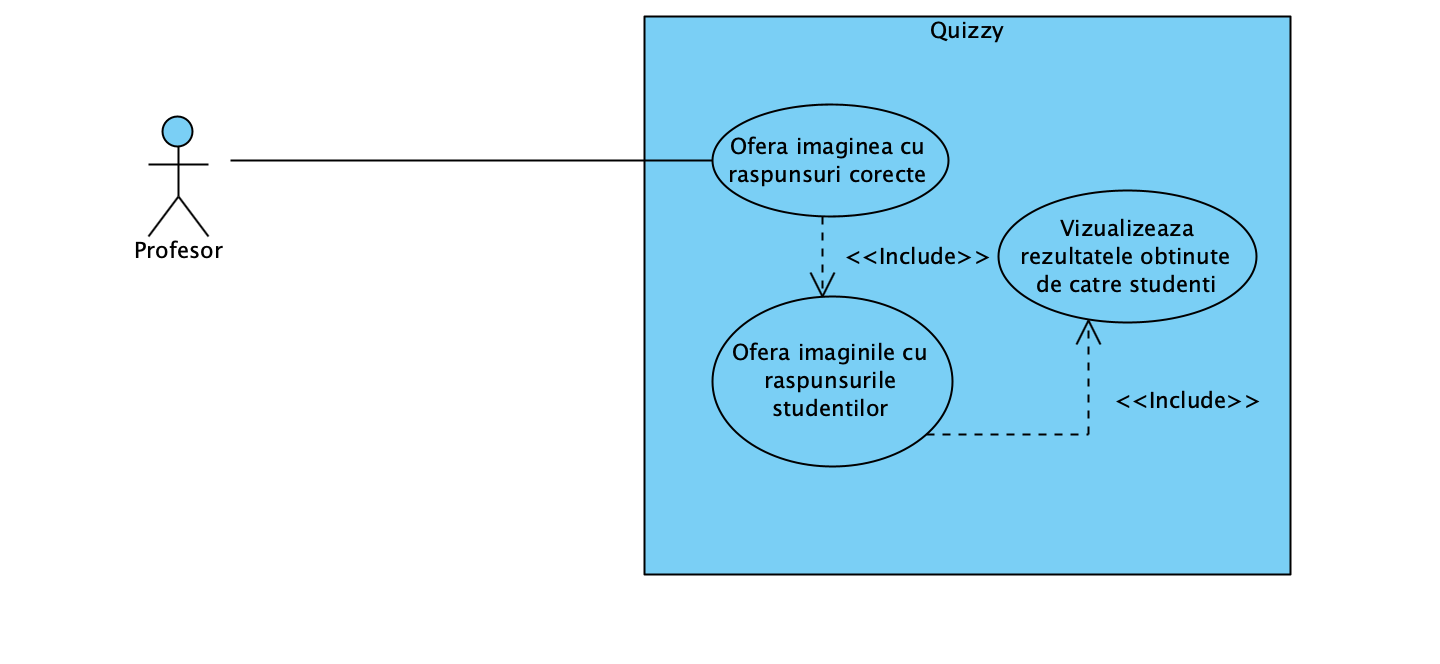
\includegraphics[width=300pt]{img/dgram1.png}
    \caption{Diagrama cazurilor de utilizare din perspectiva profesorului}
    \label{dgram1}
\end{figure}


\section{Schimburile de mesaje între utilizatorii aplica\c tiei}

Nu exist\u a schimburi de mesaje între utilizatorii aplica\c tiei, din moment ce actorul este unul singur, adic\u a profesorul.

\section{Stocarea datelor}

Stocarea datelor are loc local, în directorul proiectului, la acela\c si nivel, în 3 foldere diferite, mai precis: answers (pentru grila cu r\u aspunsurile corecte), grading (pentru grilele de r\u aspunsuri completate de studen\c ti) \c si final (pentru grilele de r\u aspunsuri corectate automat, pe baza r\u aspunsurilor oferite de studen\c ti), a\c sa cum se vede în figura \ref{datafolders}.




\begin{figure}[h!]
    \centering
    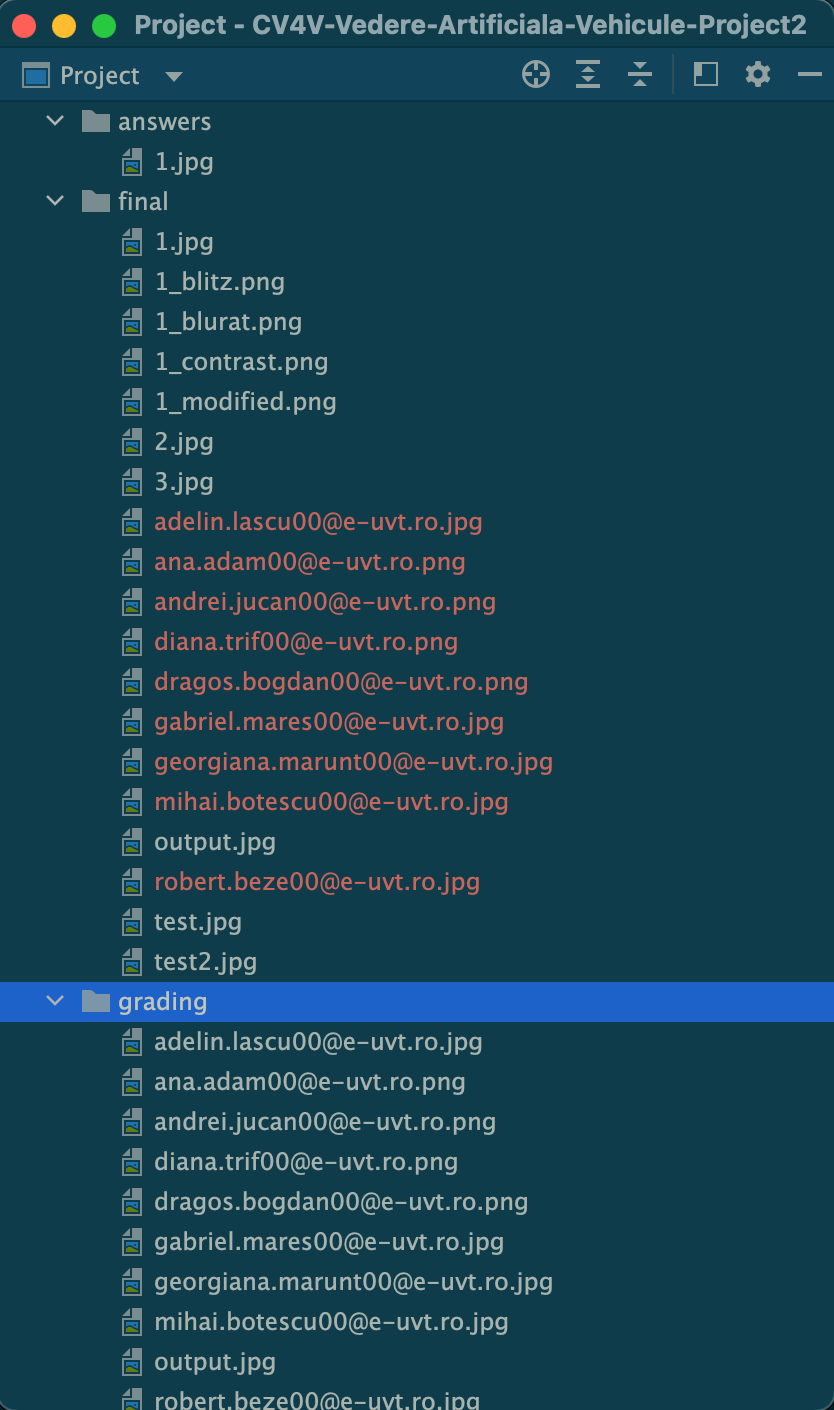
\includegraphics[width=150pt]{img/files_schema.png}
    \caption{Modalitatea de stocare a datelor}
    \label{datafolders}
\end{figure}



\newpage 

\section{Ingineria cerin\c telor}
\subsection{Cerin\c tele propuse pentru acest proiect}

\begin{enumerate}
    \item Realizarea recunoa\c sterii r\u aspunsurilor din grilele studen\c tilor
    \item Realizarea recunoa\c sterii r\u aspunsurilor din grila transmis\u a de profesor
    \item Realizarea not\u arii automate a grilelor studen\c tilor
    \item Tratarea cazurilor speciale
    \begin{itemize}
        \item Imagine foarte blurat\u a
       \item Imagine cu contrast sc\u azut
       \item Imagine cu blitz foarte puternic
     \item   Imagine cu luminozitate sc\u azut\u a
     \item   Imagine cu contrast înalt
     \item   Imagine rotit\u a
    \end{itemize}
    \item Exportarea datelor în format CSV/JSON
\end{enumerate}

\subsection{Contribu\c tii personale}
Contribu\c tiile autorilor sunt listate mai sus, exceptând punctul de plecare, adic\u a primul element enumerat.



\chapter{Tehnologii utilizate}

\section{Descrierea stivei de tehnologii}
\begin{enumerate}
    \item \textbf{Limbaj de programare}: Python3
    \item \textbf{Libr\u arii externe}: opencv \cite{DocsCV} \cite{Minichino2015-do} \cite{Bradski2017-wp} (pentru detec\c tie imagini), PIL \cite{Dey2020-cj} (pentru corec\c tie imagini), numpy \cite{DocsNumpy} (pentru procesarea imaginilor ca array-uri de pixeli)
\end{enumerate}

\section{Descrierea metodelor utilizate}

\subsection{Grayscaling}

Transform\u ari în spa\c tiul RGB \cite{DocsCV}, cum ar fi ad\u augarea/eliminarea canalului alfa, inversarea ordinii canalelor, conversia la/de la culoare RGB pe 16 bi\c ti (R5:G6:B5 sau R5:G5:B5) \cite{DocsNumpy}, precum \c si conversia în/din tonuri de gri folosind:

$$f([R,G,B]) = 0.299\cdot R+0.587\cdot G+0.114\cdot B$$

\subsection{Gaussian blur}

În aceast\u a metod\u a, în loc de un filtru box, se folose\c ste un kernel tip gaussian \cite{Minichino2015-do}. Ar trebui s\u a specific\u am l\u a\c timea \c si în\u al\c timea nucleului care ar trebui s\u a fie pozitive \c si impare. De asemenea, ar trebui s\u a specific\u am abaterea standard în direc\c tiile $X$ \c si $Y$, respectiv $sigmaX$ \c si $sigmaY$ \cite{Minichino2015-do}. Dac\u a este specificat doar $sigmaX$, $sigmaY$ este considerat la fel ca $sigmaX$. Dac\u a ambele sunt $0$, acestea sunt calculate din dimensiunea kernel-ului \cite{Bradski2017-wp}. Bluring-ul gaussian este foarte eficient în eliminarea zgomotului gaussian dintr-o imagine.

\subsection{Canny}

OpenCV pune toate cele de mai sus într-o singur\u a func\c tie, \texttt{cv.Canny()} \cite{DocsCV}. Primul argument este imaginea dorit\u a. Al doilea \c si al treilea argument sunt $minVal$ \c si, respectiv, $maxVal$ \cite{Bradski2017-wp}. Al patrulea argument este \texttt{aperture\_size}. Este dimensiunea nucleului Sobel folosit pentru g\u asirea gradien\c tilor de imagine. În mod implicit, este 3. Ultimul argument este $L2gradient$ care specific\u a ecua\c tia pentru g\u asirea m\u arimii gradientului. Dac\u a este adev\u arat, folose\c ste ecua\c tia men\c tionat\u a mai sus care este mai precis\u a, în caz contrar folose\c ste aceast\u a func\c tie: $Edge\_Gradient(G)=|Gx|+|Gy|$ \cite{Minichino2015-do}.  Am utilizat Canny pentru edge detection, în aplica\c tia noastr\u a.

\subsection{Bird's eye view (perspective)}

Bird's eye view (BEV) \cite{Bradski2017-wp} este o vedere ridicat\u a a unui obiect de sus, cu o perspectiv\u a ca \c si cum observatorul ar fi o pas\u are. Am folosit aceast\u a metod\u a pentru a putea s\u a centr\u am perspectiva asupra grilei de r\u aspunsuri.


\subsection{Treshold}

Am utilizat treshold \cite{Minichino2015-do} pentru a putea recunoa\c ste cu u\c surin\c t\u a mul\c timea tuturor r\u aspunsurilor selectate la fiecare întrebare în parte, în quiz.

\subsection{Scaling}

Am utilizat scaling pentru a realiza m\u arirea luminozit\u a\c tii imaginii în cazul în care aceasta este prea întunecat\u a.
Ne-am folosit de urm\u atoarea formul\u a, deoarece este nevoie de 2 parametri, $\alpha$ \c si $\beta$ \cite{Minichino2015-do} \cite{Bradski2017-wp}:

$$\text{ratio}=\frac{\text{brightness}}{\text{minimum-brightness}}, \alpha=\frac{1}{\text{ratio}}, \beta=255\cdot |1-\alpha|$$

,iar 

$$\text{im_nou}[x,y,z] = \alpha \cdot \text{im}[x,y,z] + \beta.$$

\chapter{Testarea aplica\c tiei}

S-au realizat multiple teste, pe cazurile speciale propuse mai sus.
Figurile \ref{t1}, \ref{t2}, \ref{t3}, \ref{t4}, \ref{t5}, \ref{t6}, \ref{t7} sugereaz\u a diferite cazuri speciale în care pot ajunge imaginile, în via\c ta real\u a.

\begin{figure}[h!]
    \centering
    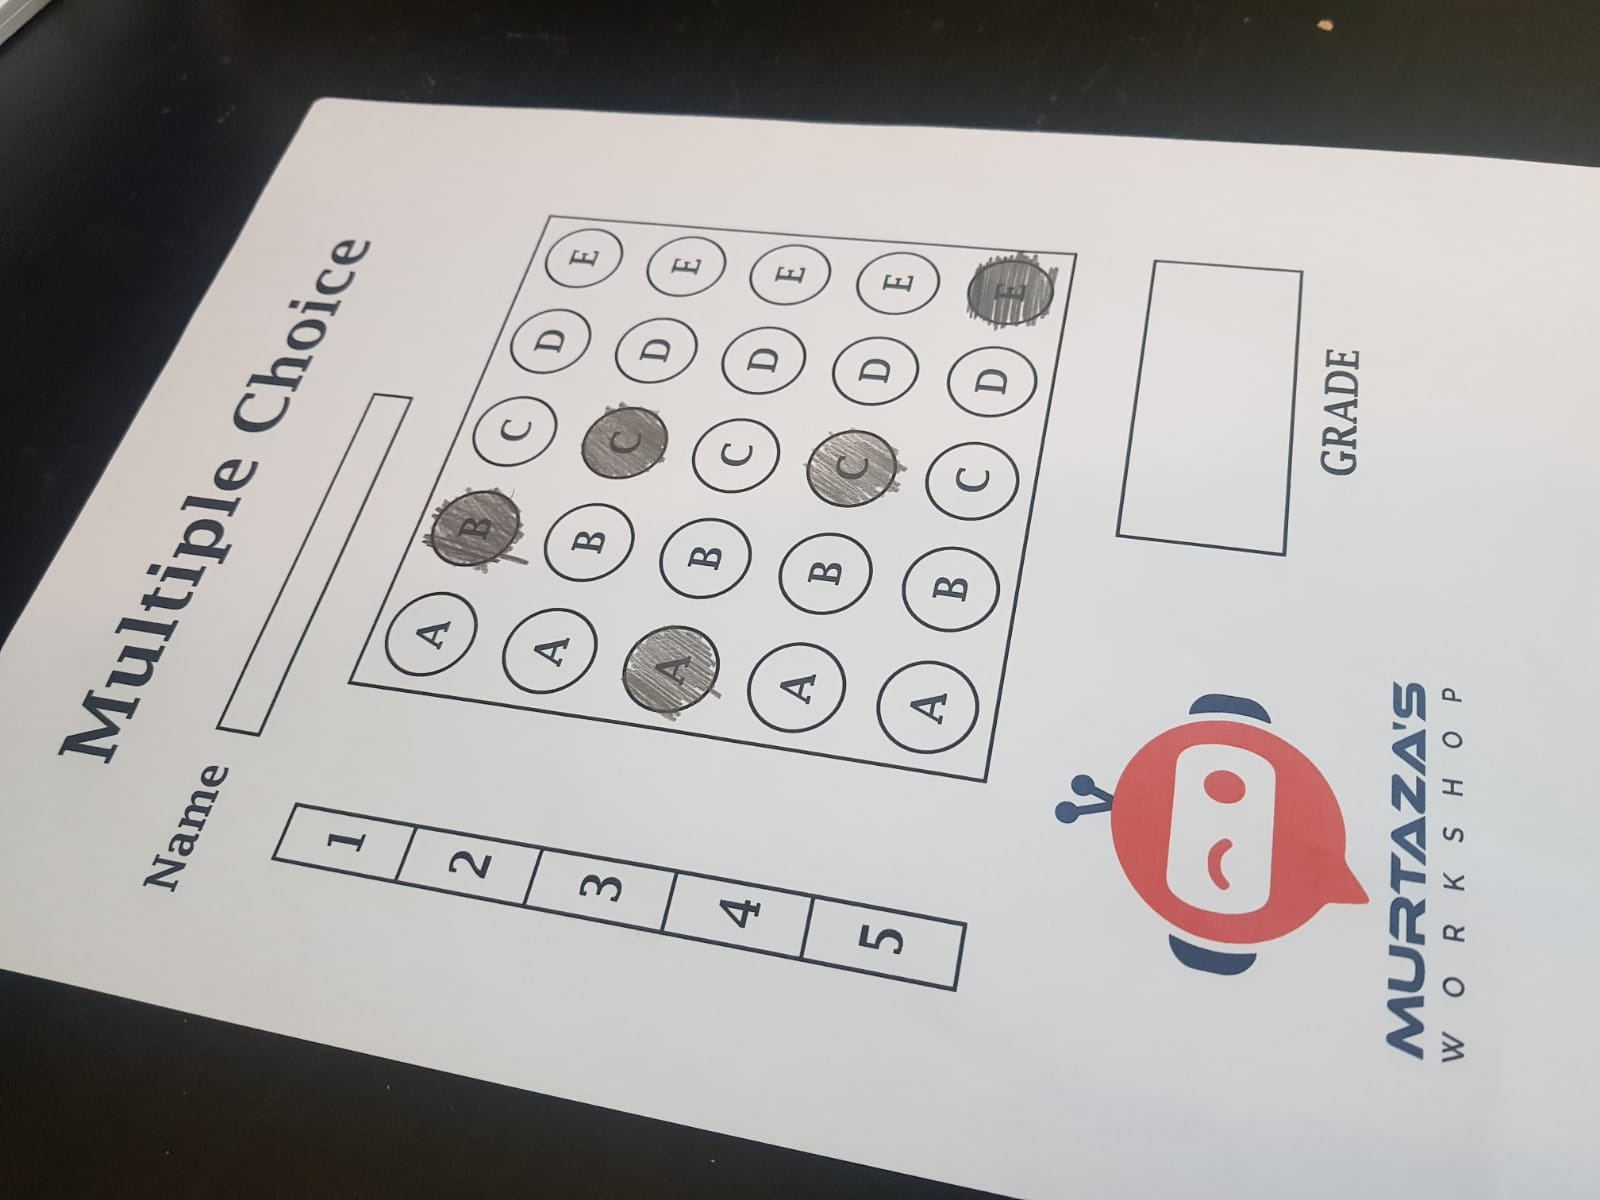
\includegraphics[width=100pt]{img/adelin.lascu00@e-uvt.ro.jpg}
    \caption{Imagine în condi\c tii normale}
    \label{t1}
\end{figure}

\begin{figure}[h!]
    \centering
    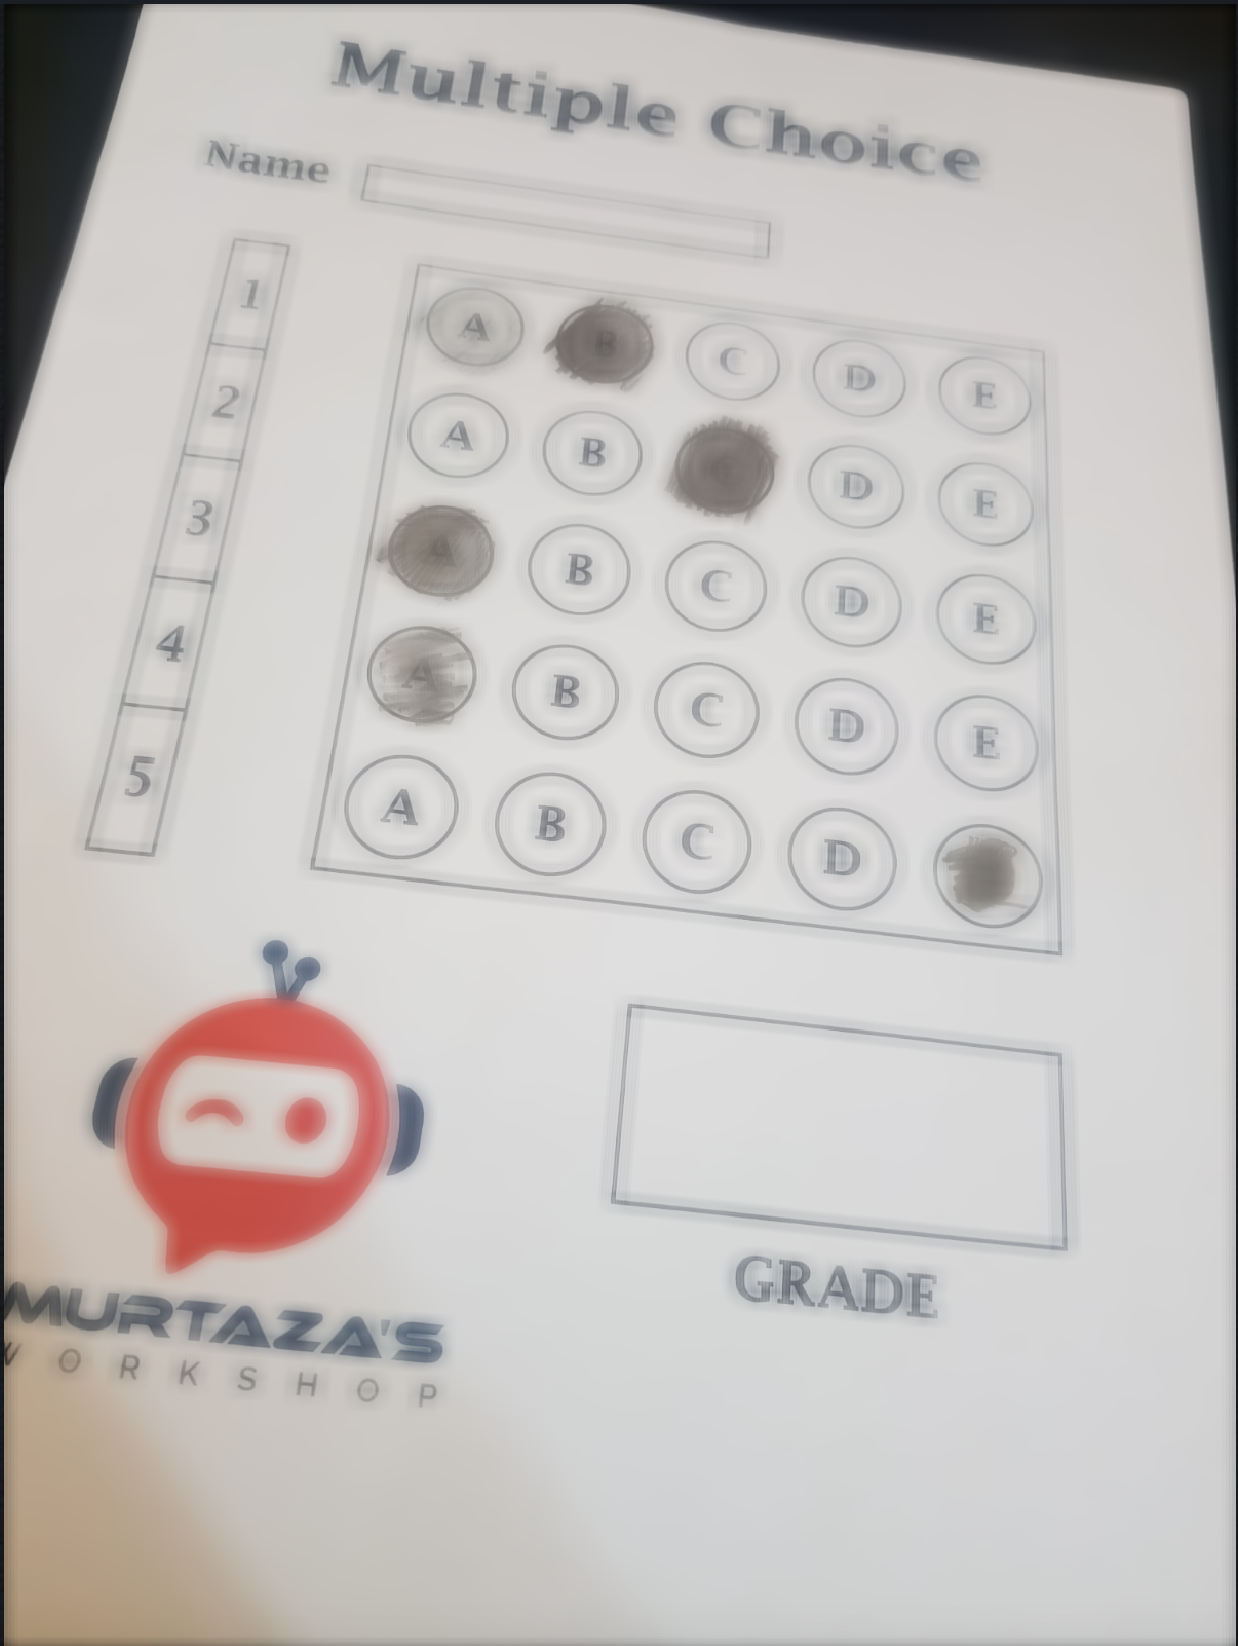
\includegraphics[width=100pt]{img/ana.adam00@e-uvt.ro.png}
    \caption{Imagine foarte blurat\u a}
    \label{t2}
\end{figure}

\begin{figure}[h!]
    \centering
    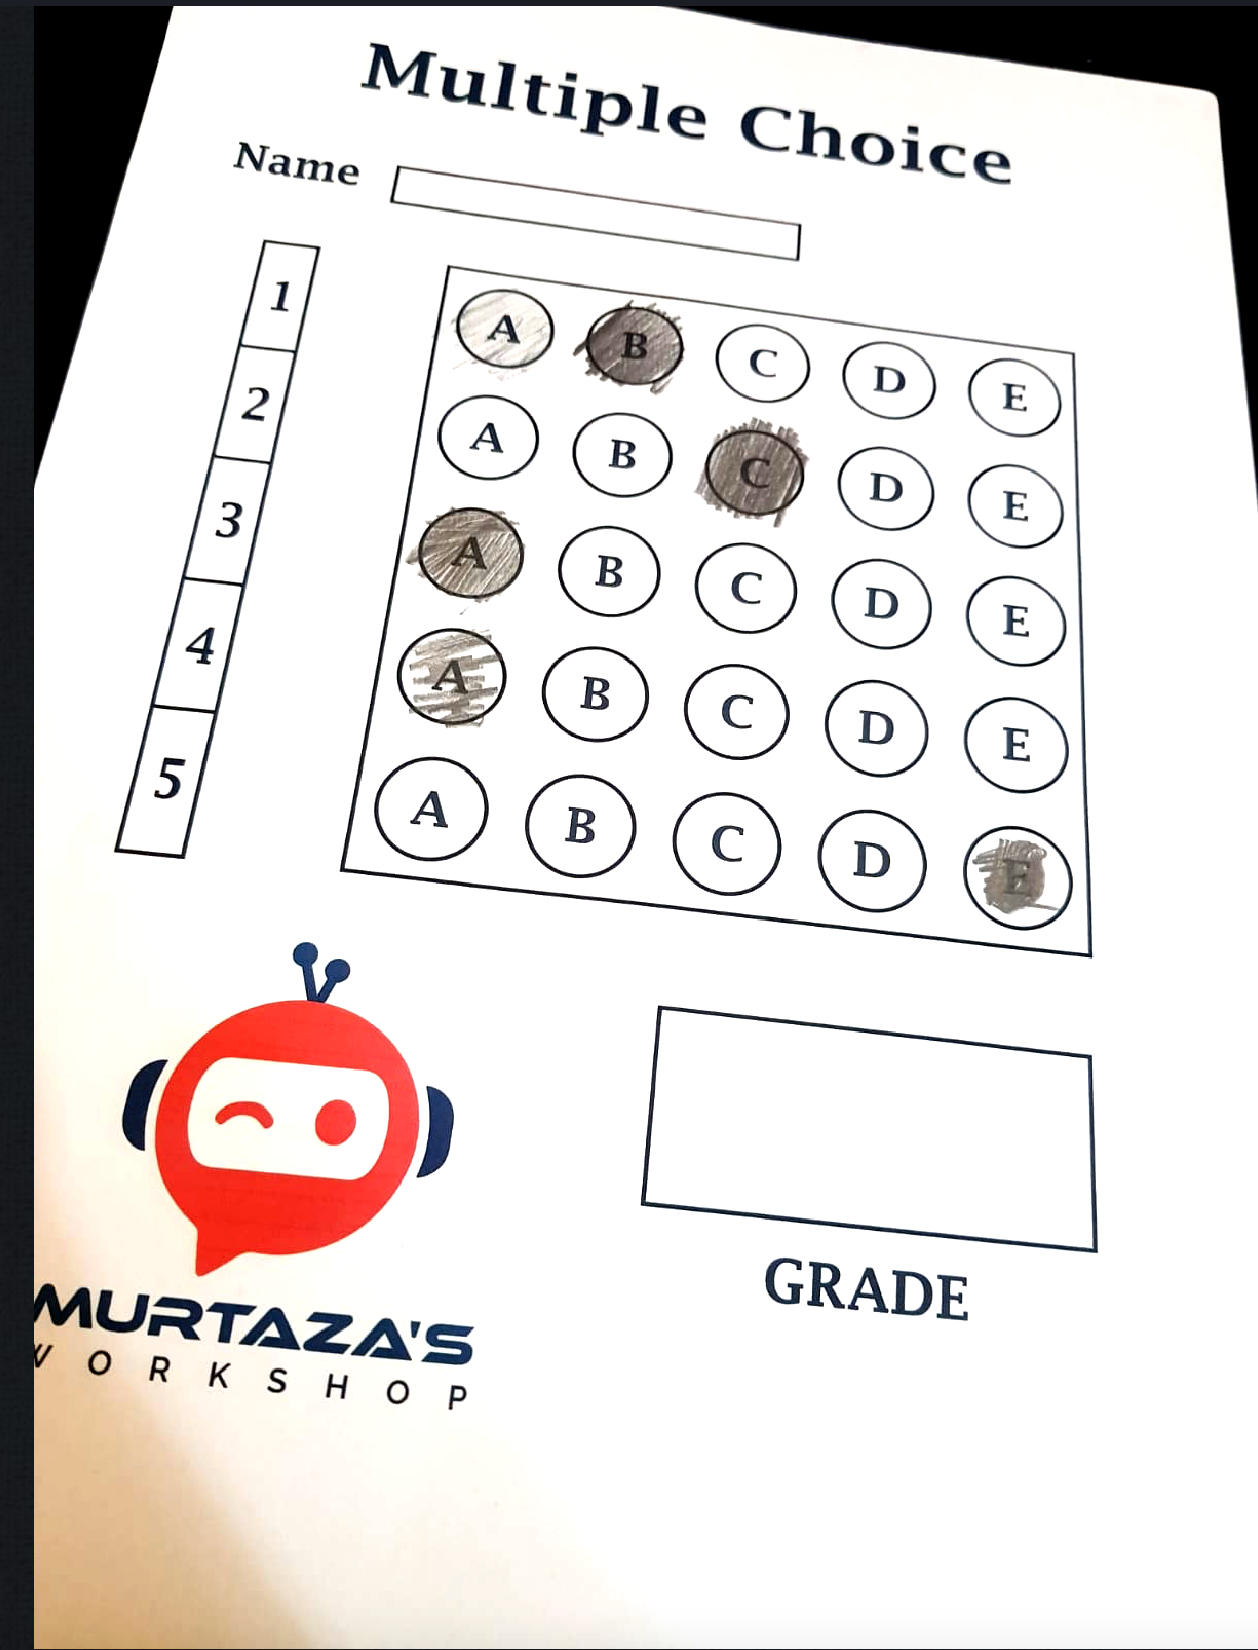
\includegraphics[width=100pt]{img/andrei.jucan00@e-uvt.ro.png}
    \caption{Imagine cu contrast sc\u azut}
    \label{t3}
\end{figure}

\begin{figure}[h!]
    \centering
    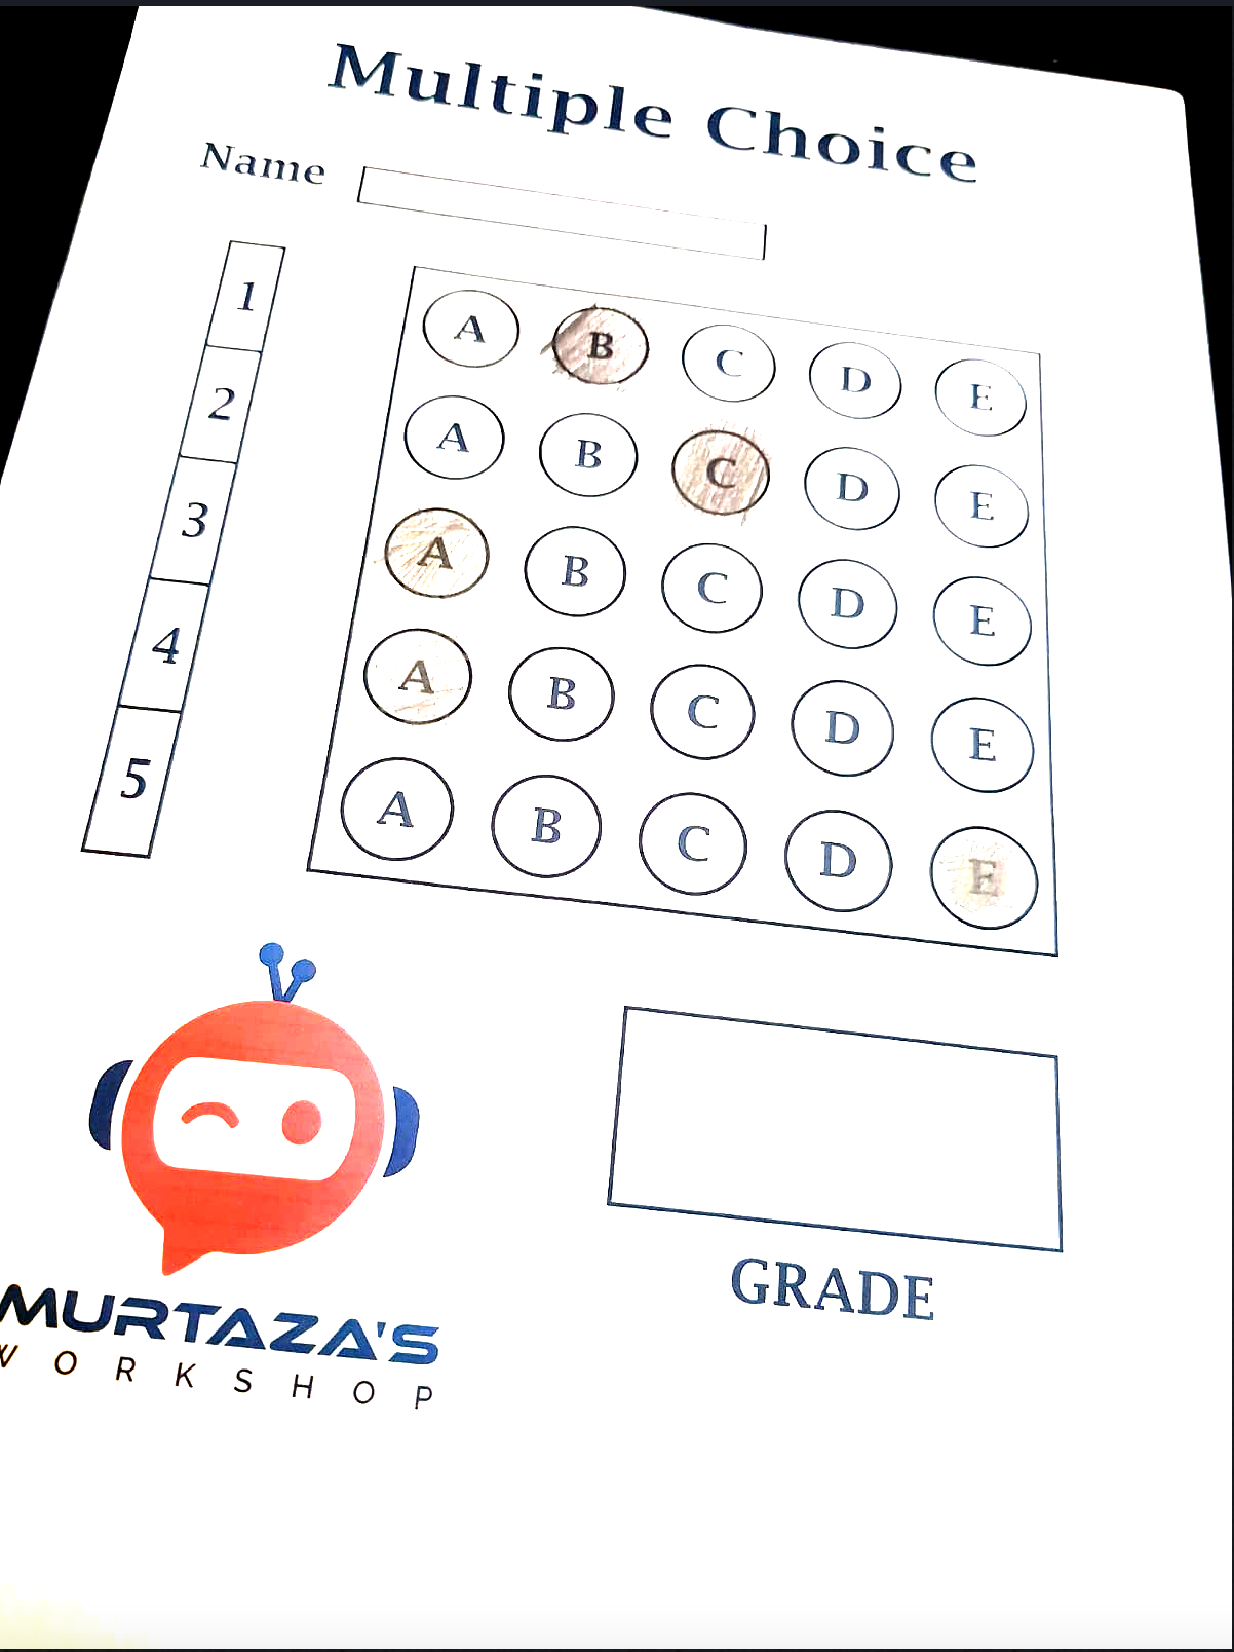
\includegraphics[width=100pt]{img/diana.trif00@e-uvt.ro.png}
    \caption{Imagine cu blitz foarte puternic}
    \label{t4}
\end{figure}

\begin{figure}[h!]
    \centering
    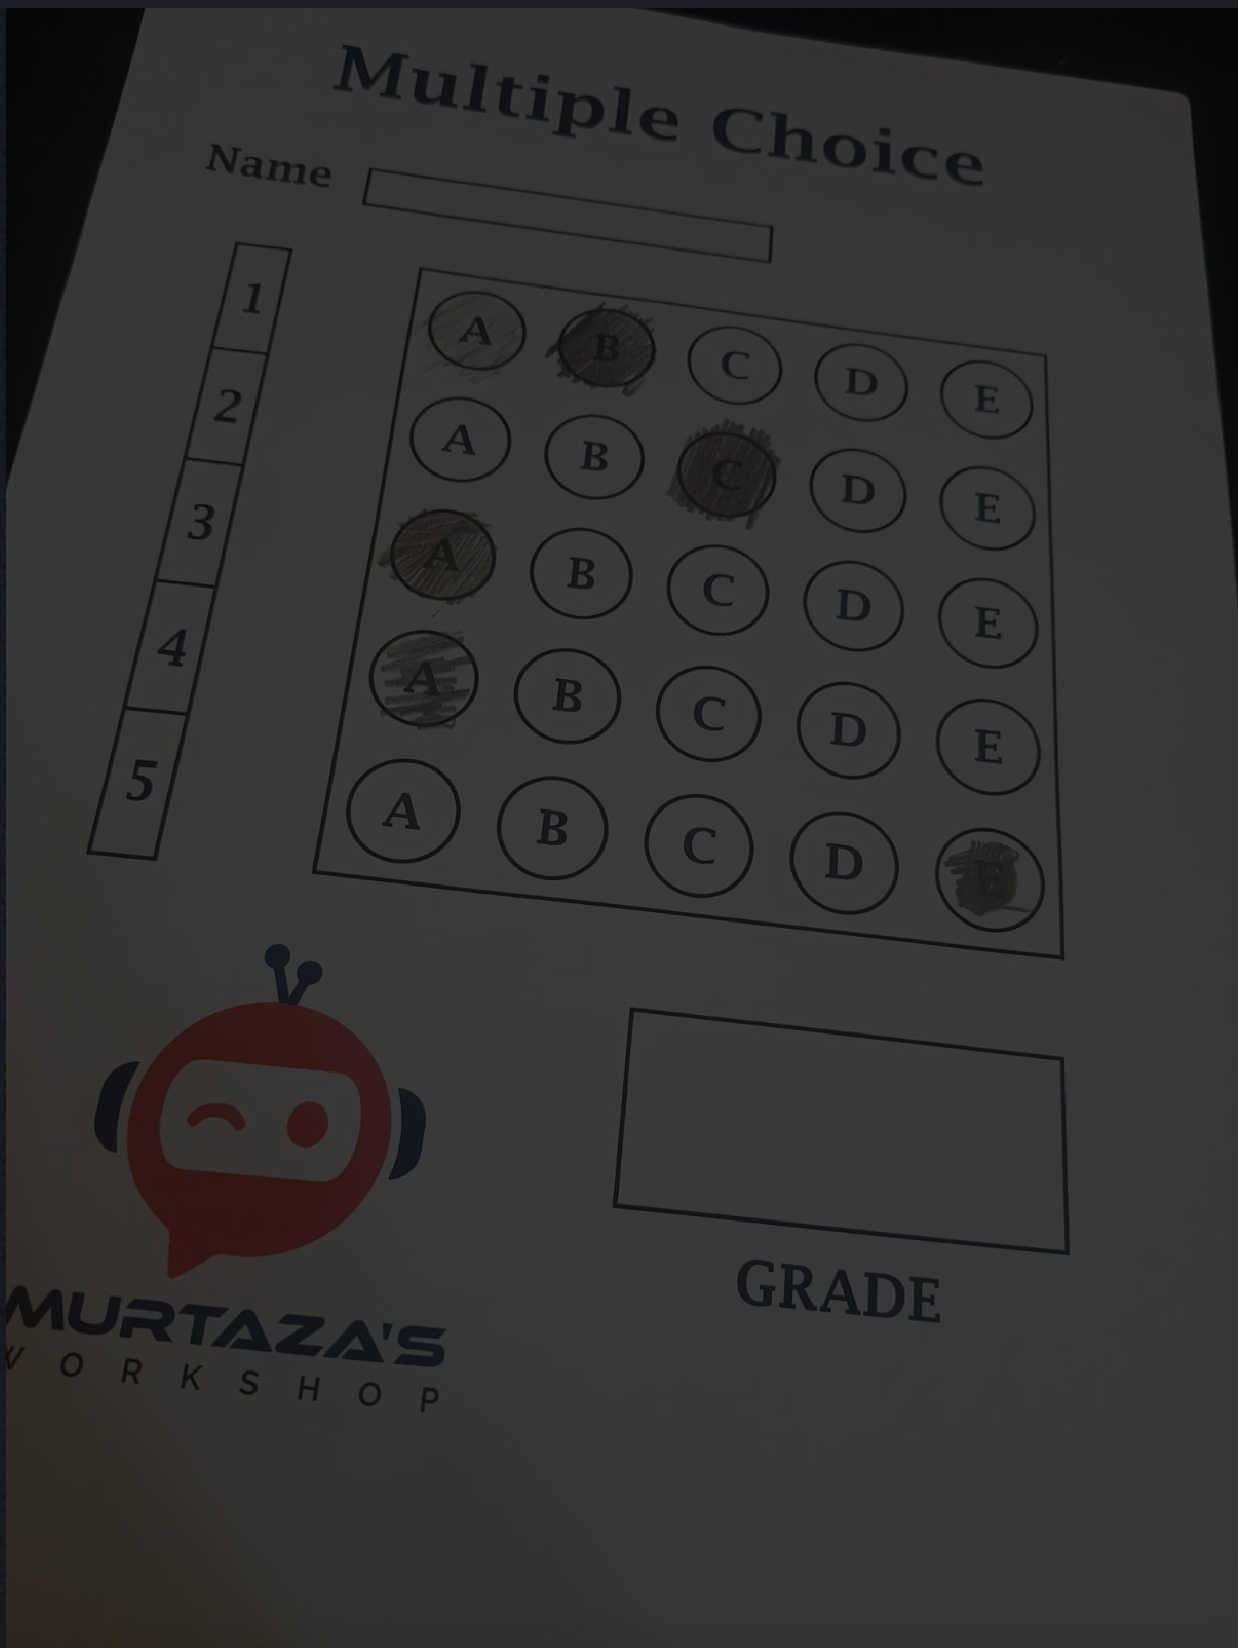
\includegraphics[width=100pt]{img/dragos.bogdan00@e-uvt.ro.png}
    \caption{Imagine cu luminozitate foarte sc\u azut\u a}
    \label{t5}
\end{figure}

\begin{figure}[h!]
    \centering
    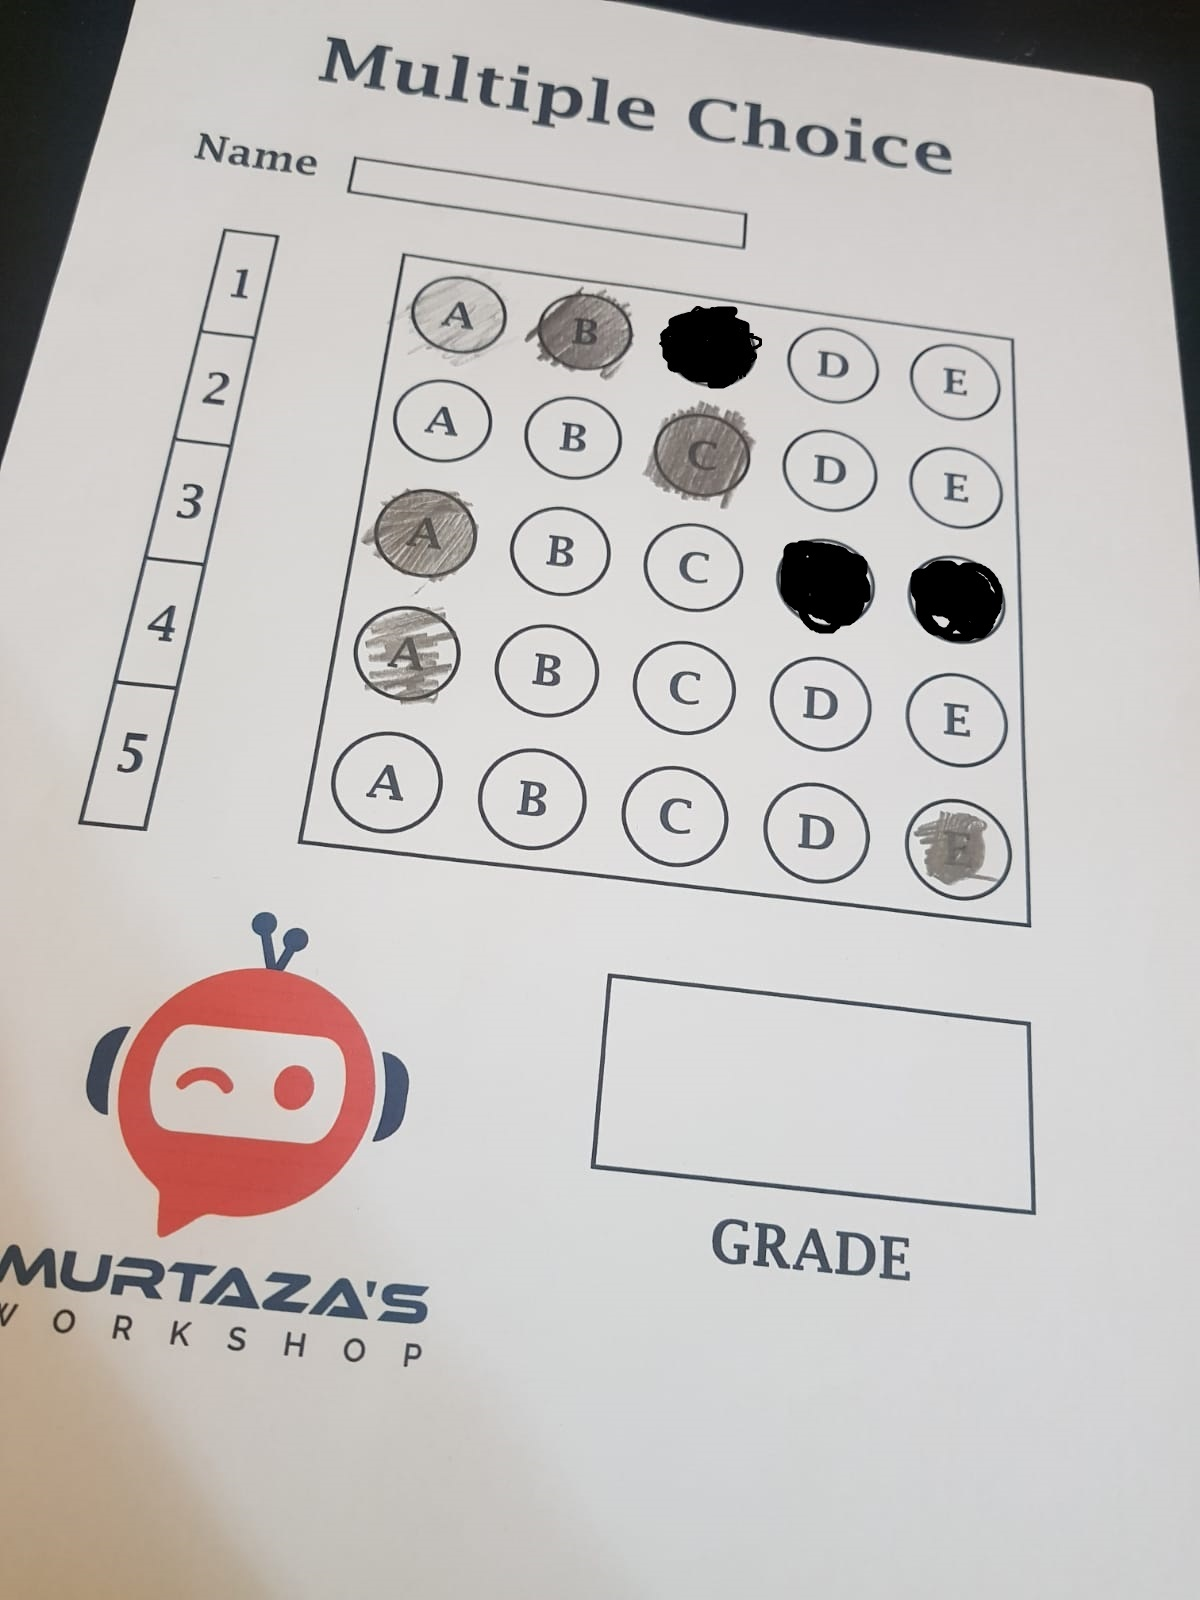
\includegraphics[width=100pt]{img/gabriel.mares00@e-uvt.ro.jpg}
    \caption{Imagine cu contrast înalt}
    \label{t6}
\end{figure}

\begin{figure}[h!]
    \centering
    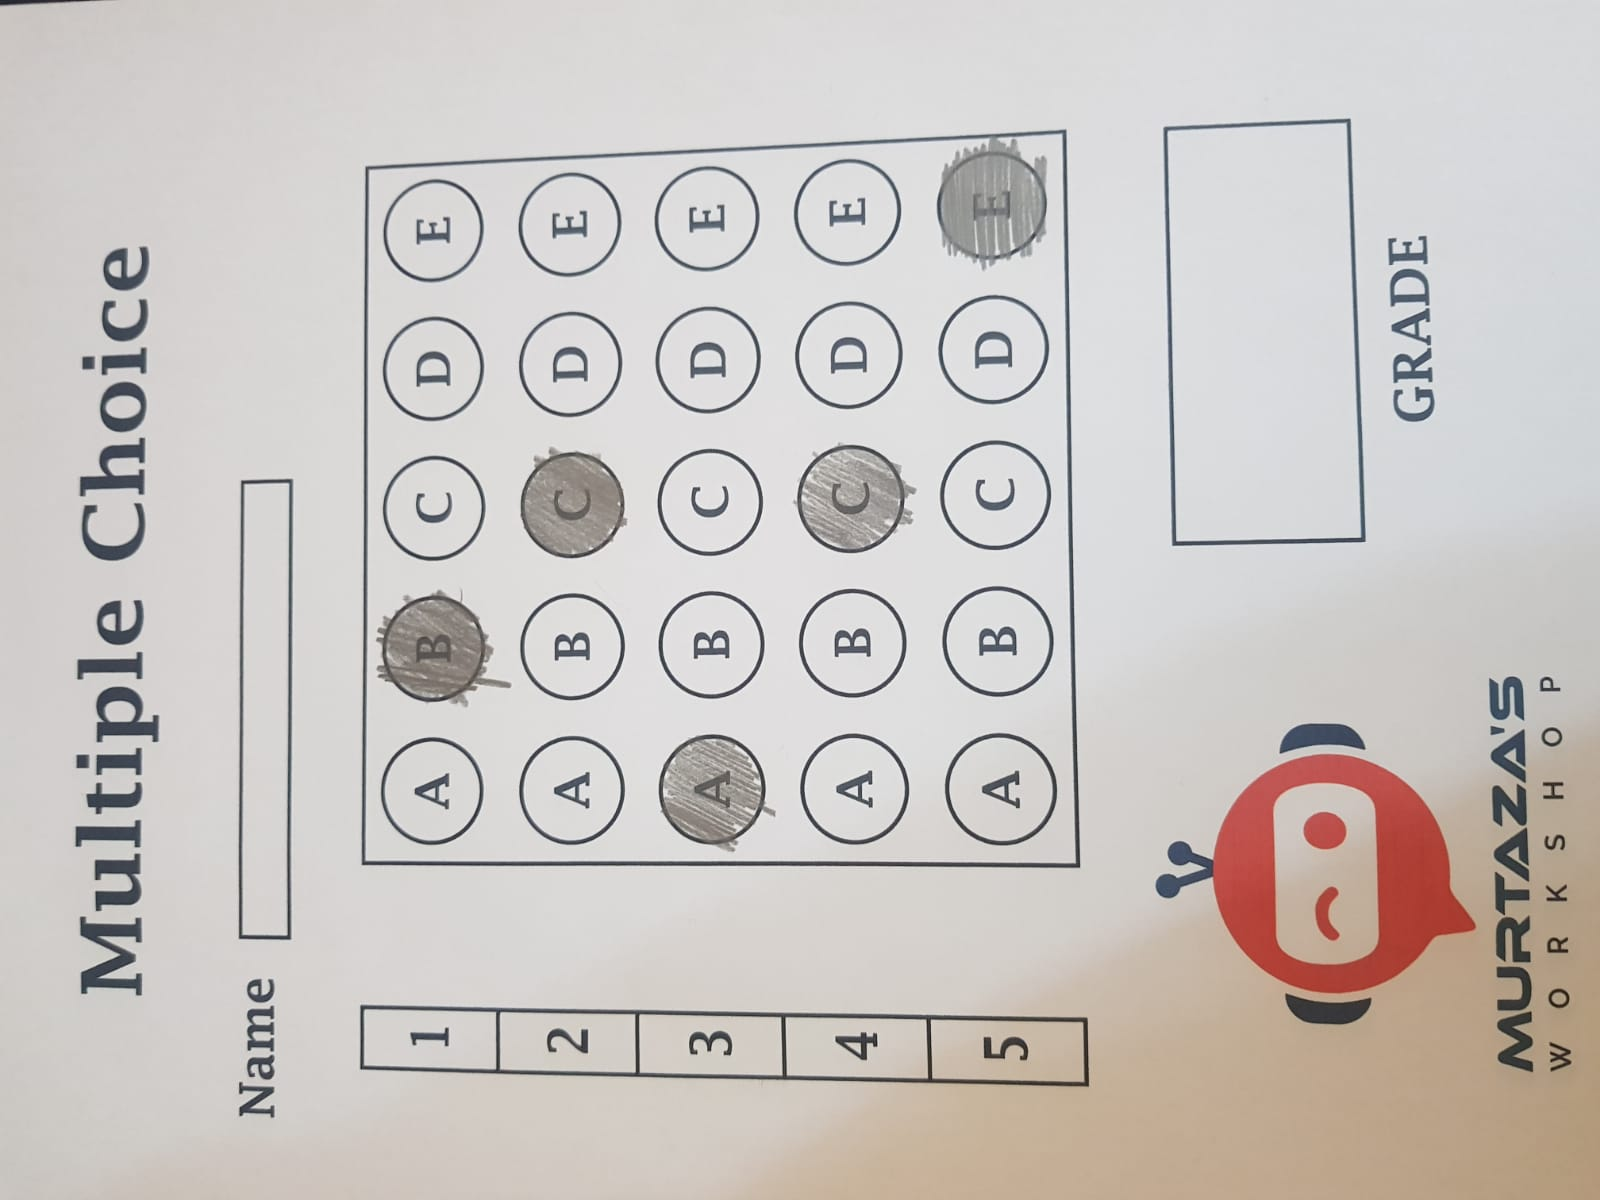
\includegraphics[width=100pt]{img/robert.beze00@e-uvt.ro.jpg}
    \caption{Imagine rotit\u a}
    \label{t7}
\end{figure}



\chapter{Concluzii \c si direc\c tii viitoare}

Ca \c si direc\c tii viitoare de realizare, se dore\c ste în primul rând extinderea aplica\c tiei spre utilizarea acesteia în mediul de web (deci creearea unui server pe care datele sunt stocate, un UI pentru interac\c tiunea dintre func\c tionalit\u a\c tile aplica\c tiei \c si utilizator), precum \c si oferirea de portabilitate acesteia.

Mai apoi, se dore\c ste identificarea \c si rezolvarea a câtor mai multe cazuri posibile care pot ap\u area în momentul fotografierii grilelor.

De asemenea, posibilitate de extindere pentru a func\c tiona \c si pe un alt \c sablon decât cel oferit în momentul de fa\c t\u a.

Se dore\c ste \c si posibilitatea \c si de recunoa\c stere a email-ului studentului din cadrul imaginilor scanate. 

	\bibliography{mybib}
		\bibliographystyle{ieeetr}
		\addcontentsline{toc}{chapter}{Bibliografie}




\end{document}
